%% —-----------------------------------------------------------
%% main.tex — Proposta de Portfólio (PAC 8)
%% Sistema Multiagente Inteligente de Cobrança com LLM, RAG e ML
%% Template SBC Reviews 2025 (CC BY 4.0) — Sociedade Brasileira de Computação.
%% Compilação: xelatex main -> bibtex main -> xelatex main -> xelatex main
%% —-----------------------------------------------------------

\documentclass[portuguese]{sbcreviews-2025}%

%\usepackage{graphicx}  % carregada dentro da classe
%\usepackage{fontspec}  % carregada dentro da classe
%\usepackage{fontawesome}
%\usepackage{color}
%\usepackage{hyperref}

\usepackage{aas_macros}
\usepackage[bottom]{footmisc}

\usepackage{tabularray}
\usepackage{afterpage}
\usepackage{url}
\usepackage{xurl}   % permite quebra de URLs longas (refer\^encias)
\usepackage{pifont}

\usepackage{tikz}
\usetikzlibrary{arrows.meta, positioning, fit, backgrounds}

% apalike-sol gera entradas no formato [Autor, Ano] (apalike clássico, não-natbib);
% colocamos o natbib em modo numérico para citações [n] consistentes e sem erro de parsing.
\setcitestyle{numbers,square,comma}

\definecolor{engtitle}{rgb}{0.5,0.5,0.5}
\definecolor{orcidlogo}{rgb}{0.37,0.48,0.13}
\definecolor{unilogo}{rgb}{0.16, 0.26, 0.58}
\definecolor{maillogo}{rgb}{0.58, 0.16, 0.26}
\definecolor{darkblue}{rgb}{0.0,0.0,0.0}
\hypersetup{colorlinks,breaklinks,
            linkcolor=darkblue,urlcolor=darkblue,
            anchorcolor=darkblue,citecolor=darkblue}

%% Símbolos da tabela comparativa
\newcommand{\atende}{\textcolor{green!55!black}{\ding{51}}}
\newcommand{\parcial}{\textcolor{orange!90!black}{$\sim$}}
\newcommand{\naoatende}{\textcolor{red!70!black}{\ding{55}}}

\jid{ROCS}
\jtitle{SBC Computing Reviews, 202X, XX:1}
\issn{2966-3938}
\doi{10.5753/rocs.202X.XXXXXX}
\copyrightstatement{This work is licensed under a Creative Commons Attribution 4.0 International License}
\jyear{202X}

\category{Proposta de Portfólio}
\title[Sistema Multiagente Inteligente de Cobrança]{Sistema Multiagente Inteligente de Cobrança com LLM, RAG e Machine Learning}
\engtitle{\textcolor{engtitle}{Intelligent Multi-Agent Collection System with LLM, RAG and Machine Learning}}

\author[Rocha 2026]{
\affil{\textbf{Gabriel Forster Rocha}~\textcolor{blue}{\faEnvelope}~~[{Centro Universit\'ario Cat\'olica de Santa Catarina}~|\href{mailto:gabriel04.rocha@catolicasc.edu.br}{~{\textit{gabriel04.rocha@catolicasc.edu.br}}}~]}

\affil{\textbf{Andrei Carniel}~\textcolor{blue}{\faEnvelope}~~[{Centro Universit\'ario Cat\'olica de Santa Catarina}~|\href{mailto:andrei.carniel@catolicasc.org.br}{~{\textit{andrei.carniel@catolicasc.org.br}}}~]}
}

\begin{document}

\begin{frontmatter}

\maketitle

\begin{mail}
Curso de Engenharia de Software, Centro Universit\'ario --- Cat\'olica de Santa Catarina, Jaragu\'a do Sul, SC, Brasil.
\end{mail}

\begin{abstract-pt}
Este trabalho prop\~oe o desenvolvimento de um sistema multiagente inteligente de cobran\c{c}a que integra modelos de linguagem de grande escala (\textit{Large Language Models} --- LLMs), gera\c{c}\~ao aumentada por recupera\c{c}\~ao (\textit{Retrieval-Augmented Generation} --- RAG), modelos preditivos de \textit{Machine Learning} e servi\c{c}os de processamento de voz. O sistema opera em dois modos complementares: (i) um modo responsivo, no qual o agente utiliza RAG para responder d\'uvidas de clientes com base em documenta\c{c}\~ao interna; e (ii) um modo ativo (proativo), no qual o pr\'oprio sistema identifica documentos vencidos ou clientes inadimplentes e inicia a abordagem de cobran\c{c}a de forma aut\^onoma, inclusive por chamadas telef\^onicas automatizadas. Um m\'odulo preditivo classifica clientes por propens\~ao ao pagamento e antecipa a inadimpl\^encia futura, possibilitando cobran\c{c}a preventiva. Diante de um cen\'ario de inadimpl\^encia que afeta dezenas de milh\~oes de consumidores no Brasil, os processos tradicionais de cobran\c{c}a apresentam limita\c{c}\~oes de escalabilidade, personaliza\c{c}\~ao e tempestividade. A combina\c{c}\~ao de agentes aut\^onomos, modelos de linguagem e aprendizado de m\'aquina representa, portanto, uma oportunidade relevante para automatizar e otimizar o ciclo de recupera\c{c}\~ao de cr\'edito em m\'ultiplos canais. Este documento apresenta a proposta de portf\'olio, descrevendo o problema de pesquisa, a hip\'otese, os objetivos, a inova\c{c}\~ao, a arquitetura e as tecnologias previstas, os resultados esperados e o cronograma de desenvolvimento.
\end{abstract-pt}

\begin{abstract-en}
This work proposes the development of an intelligent multi-agent collection system that integrates Large Language Models (LLMs), Retrieval-Augmented Generation (RAG), predictive Machine Learning models, and voice processing services. The system operates in two complementary modes: (i) a responsive mode, in which the agent uses RAG to answer customer questions based on internal documentation; and (ii) an active (proactive) mode, in which the system itself identifies overdue documents or delinquent customers and autonomously initiates the collection approach, including automated phone calls. A predictive module classifies customers by their propensity to pay and anticipates future delinquency, enabling preventive collection. Given a delinquency scenario affecting tens of millions of consumers in Brazil, traditional collection processes show limitations in scalability, personalization, and timeliness. Combining autonomous agents, language models, and machine learning thus represents a relevant opportunity to automate and optimize the credit recovery cycle across multiple channels. This document presents the portfolio proposal, describing the research problem, the hypothesis, the objectives, the innovation, the planned architecture and technologies, the expected results, and the development schedule.
\end{abstract-en}

\begin{pchaves}
Sistema multiagente, Intelig\^encia Artificial, Cobran\c{c}a automatizada, RAG, Machine Learning, LLM
\end{pchaves}

\begin{keywords}
Multi-agent system, Artificial Intelligence, Automated collection, RAG, Machine Learning, LLM
\end{keywords}

\end{frontmatter}

%% ============================================================
%%  1. INTRODUÇÃO
%% ============================================================
\section{Introdu\c{c}\~ao}
\label{sec:intro}

O cen\'ario de inadimpl\^encia no Brasil apresenta desafios estruturais significativos para empresas de todos os portes. Dezenas de milh\~oes de brasileiros encontram-se em situa\c{c}\~ao de inadimpl\^encia, o que impacta diretamente o fluxo de caixa das organiza\c{c}\~oes e eleva os custos operacionais associados \`a recupera\c{c}\~ao de cr\'edito \cite{serasa2024}. Nesse contexto, os processos tradicionais de cobran\c{c}a --- baseados em liga\c{c}\~oes manuais, envio de correspond\^encias e negocia\c{c}\~oes presenciais --- revelam-se cada vez mais insuficientes diante do volume crescente de devedores e da necessidade de abordagens personalizadas e tempestivas \cite{cnc2025}.

Paralelamente, os avan\c{c}os recentes em Intelig\^encia Artificial (IA) t\^em proporcionado novas possibilidades para a automa\c{c}\~ao de processos complexos que envolvem linguagem natural e tomada de decis\~ao. Destacam-se os \textit{Large Language Models} (LLMs), capazes de compreender e gerar texto com elevado grau de coer\^encia e adequa\c{c}\~ao contextual \cite{brown2020language}. Complementarmente, a t\'ecnica de \textit{Retrieval-Augmented Generation} (RAG) permite que esses modelos consultem bases de conhecimento externas antes de formular uma resposta, reduzindo alucina\c{c}\~oes e aumentando a precis\~ao das informa\c{c}\~oes fornecidas \cite{lewis2020retrieval}. Al\'em disso, abordagens de \textit{Machine Learning} (ML) possibilitam a constru\c{c}\~ao de modelos preditivos que identificam padr\~oes em dados hist\'oricos para antecipar comportamentos futuros, como a propens\~ao de um cliente a quitar ou n\~ao uma d\'ivida \cite{hastie2009elements}. No dom\'inio de sistemas inteligentes, o paradigma de \textit{agentes aut\^onomos} e \textit{sistemas multiagentes} tem ganhado relev\^ancia pr\'atica: diferentemente de aplica\c{c}\~oes conversacionais passivas, agentes aut\^onomos planejam, executam a\c{c}\~oes e interagem com ferramentas externas de forma independente, orientados por objetivos \cite{wang2024survey}. A isso soma-se a integra\c{c}\~ao de servi\c{c}os de voz: tecnologias de transcri\c{c}\~ao autom\'atica de fala, como o Whisper \cite{radford2023robust} e o Google Speech-to-Text \cite{google2024stt}, e plataformas de telefonia program\'avel, como Twilio \cite{twilio2024docs}, ampliam os canais de comunica\c{c}\~ao dispon\'iveis para sistemas automatizados.

Diante desse panorama, o presente trabalho prop\~oe um sistema multiagente inteligente de cobran\c{c}a que integra LLMs, RAG, modelos preditivos de ML e servi\c{c}os de voz, operando de forma responsiva e proativa para automatizar o ciclo de recupera\c{c}\~ao de cr\'edito em m\'ultiplos canais.

A relev\^ancia do trabalho decorre do impacto econ\^omico da inadimpl\^encia e da lacuna observada nas solu\c{c}\~oes existentes: ferramentas comerciais e acad\^emicas atacam aspectos isolados do problema --- ou a previs\~ao de risco, ou a automa\c{c}\~ao por voz, ou o atendimento conversacional --- mas n\~ao integram, em um \'unico fluxo, intelig\^encia preditiva, recupera\c{c}\~ao de conhecimento e opera\c{c}\~ao multicanal. Ao reunir essas capacidades, a proposta busca tanto reduzir o custo operacional da cobran\c{c}a quanto qualificar o contato com o cliente, direcionando o esfor\c{c}o humano para os casos de maior complexidade.

\textit{Problema de Pesquisa:} os m\'etodos convencionais de cobran\c{c}a enfrentam limita\c{c}\~oes de escalabilidade, personaliza\c{c}\~ao e tempestividade. Operadores humanos possuem capacidade limitada de atendimento simult\^aneo, e a aus\^encia de prioriza\c{c}\~ao inteligente frequentemente direciona esfor\c{c}os a clientes com baixa probabilidade de pagamento, enquanto devedores com maior propens\~ao \`a quita\c{c}\~ao permanecem sem contato adequado \cite{thomas2009credit}. Formula-se, assim, a pergunta: \textit{em que medida um sistema multiagente inteligente, baseado em LLMs com RAG e modelos preditivos de Machine Learning, integrado a servi\c{c}os de transcri\c{c}\~ao de \'audio e telefonia program\'avel, \'e capaz de automatizar o processo de cobran\c{c}a --- tanto de forma responsiva quanto proativa --- e contribuir para o aumento da efici\^encia na recupera\c{c}\~ao de cr\'edito em compara\c{c}\~ao com abordagens convencionais?}

\textit{Hip\'otese:} um sistema multiagente que combine (i) agentes conversacionais baseados em LLMs com RAG para atendimento responsivo, (ii) agentes aut\^onomos para abordagem proativa por m\'ultiplos canais (texto, \'audio e chamadas telef\^onicas) e (iii) um m\'odulo preditivo de ML para classifica\c{c}\~ao de inadimplentes e previs\~ao de inadimpl\^encia futura \'e capaz de reduzir o tempo m\'edio de recupera\c{c}\~ao de cr\'edito e aumentar a taxa de resolu\c{c}\~ao de pend\^encias financeiras, quando comparado a processos manuais ou parcialmente automatizados sem intelig\^encia preditiva \cite{lessmann2015benchmarking}.

\textit{Objetivos:} o objetivo geral \'e desenvolver e avaliar um sistema multiagente inteligente de cobran\c{c}a que integre LLMs com RAG, agentes aut\^onomos, modelos preditivos de ML e servi\c{c}os de voz, operando de forma responsiva e proativa. Como objetivos espec\'ificos pretende-se: (a) analisar os processos tradicionais de cobran\c{c}a e levantar requisitos, considerando aspectos legais e operacionais; (b) projetar a arquitetura multiagente e os mecanismos de coordena\c{c}\~ao entre os agentes; (c) implementar o m\'odulo responsivo com LLM e RAG; (d) implementar o m\'odulo ativo com agentes aut\^onomos e integra\c{c}\~ao a canais de voz; (e) desenvolver o m\'odulo preditivo de ML para classifica\c{c}\~ao e previs\~ao de inadimpl\^encia; e (f) avaliar o sistema por meio de experimentos controlados, com m\'etricas preditivas e indicadores operacionais comparados a \textit{baselines}.

\textit{Estrutura\c{c}\~ao do Texto:} a Se\c{c}\~ao~\ref{sec:tr} discute os trabalhos relacionados; a Se\c{c}\~ao~\ref{sec:metodologia} apresenta a proposta, a inova\c{c}\~ao e a arquitetura e tecnologias; a Se\c{c}\~ao~\ref{sec:resultados} descreve os resultados esperados; a Se\c{c}\~ao~\ref{sec:discconclusao} traz discuss\~oes e conclus\~oes; e o Ap\^endice (Se\c{c}\~ao~\ref{sec:apendice}) re\'une a tabela comparativa e o cronograma de desenvolvimento.

%% ============================================================
%%  2. TRABALHOS RELACIONADOS
%% ============================================================
\section{Trabalhos Relacionados}
\label{sec:tr}

A literatura e o mercado oferecem contribui\c{c}\~oes parciais ao problema abordado. No eixo acad\^emico, \citet{wang2024survey} apresentam uma revis\~ao sistem\'atica sobre agentes aut\^onomos baseados em LLMs, fundamentando o paradigma multiagente adotado neste trabalho, embora sem foco em cobran\c{c}a. \citet{mestiri2024credit} aplica modelos de \textit{Machine Learning} e \textit{Deep Learning} \`a tarefa de \textit{credit scoring}, evidenciando o potencial preditivo em cr\'edito, por\'em sem componente conversacional ou multicanal. Mais pr\'oximo da proposta, o sistema MASCA \cite{jajoo2025masca} combina m\'ultiplos agentes baseados em LLMs para avalia\c{c}\~ao de cr\'edito, mas n\~ao trata da execu\c{c}\~ao da cobran\c{c}a nem da opera\c{c}\~ao por voz.

Entre as solu\c{c}\~oes comerciais, o HighRadius \cite{highradius} \'e uma plataforma de automa\c{c}\~ao de cobran\c{c}a apoiada em IA e ML voltada predominantemente a canais textuais, enquanto Skit.ai \cite{skitai} e Tovie AI \cite{tovieai} oferecem cobran\c{c}a automatizada por voz, integrando LLMs, telefonia program\'avel e transcri\c{c}\~ao autom\'atica de fala. Nenhuma dessas solu\c{c}\~oes, contudo, re\'une simultaneamente RAG, arquitetura multiagente, opera\c{c}\~ao multicanal (texto e voz) e cobran\c{c}a preventiva baseada em previs\~ao de inadimpl\^encia futura. A an\'alise comparativa detalhada, com 12 crit\'erios, \'e apresentada na Tabela~\ref{tab:comparativa} (Ap\^endice, Se\c{c}\~ao~\ref{sec:apendice}).

%% ============================================================
%%  3. METODOLOGIA
%% ============================================================
\section{Metodologia}
\label{sec:metodologia}

A pesquisa \'e de natureza aplicada, com abordagem experimental e desenvolvimento incremental, organizado em quatro etapas: (i) levantamento de requisitos funcionais e n\~ao funcionais e an\'alise do dom\'inio, incluindo aspectos legais --- C\'odigo de Defesa do Consumidor \cite{cdc1990}, LGPD \cite{lgpd2018} e regras do PROCON quanto a hor\'ario e frequ\^encia de contato; (ii) projeto da arquitetura multiagente; (iii) implementa\c{c}\~ao dos m\'odulos; e (iv) avalia\c{c}\~ao por experimentos controlados frente a \textit{baselines} convencionais. As fontes de dados para os modelos preditivos compreendem o hist\'orico de clientes e documentos financeiros (dados cadastrais, vencimentos, pagamentos, atrasos e acordos), anonimizados conforme a LGPD e divididos em treino, valida\c{c}\~ao e teste (70/15/15) com estratifica\c{c}\~ao e respeito \`a ordem temporal para evitar vazamento de dados. A base de conhecimento do RAG \'e composta por pol\'iticas internas, \textit{scripts} de negocia\c{c}\~ao, tabelas de parcelamento e FAQs, fragmentados em \textit{chunks} e indexados em banco vetorial.

\subsection{Proposta de Portf\'olio}
\label{sec:proposta}

Prop\~oe-se um sistema organizado em tr\^es m\'odulos que operam de forma coordenada sob um orquestrador central.

O \textbf{m\'odulo responsivo} (LLM + RAG) \'e acionado quando o cliente entra em contato por texto ou \'audio; mensagens de voz do WhatsApp s\~ao transcritas por um servi\c{c}o de \textit{speech-to-text} antes do processamento. O agente identifica a inten\c{c}\~ao do cliente --- consulta de d\'ebito, segunda via, negocia\c{c}\~ao/parcelamento, contesta\c{c}\~ao ou confirma\c{c}\~ao de pagamento --- e, por meio do \textit{pipeline} RAG, recupera os fragmentos mais relevantes da base de conhecimento (busca por similaridade de cosseno sobre \textit{embeddings}, sele\c{c}\~ao dos \textit{top-k} trechos e \textit{re-ranking} opcional). Esses trechos, somados aos dados do cliente e ao hist\'orico da conversa, comp\~oem o \textit{prompt} enviado ao LLM, que gera uma resposta ancorada exclusivamente na documenta\c{c}\~ao interna. Crit\'erios de escala\c{c}\~ao --- pedido expl\'icito do cliente, baixa confian\c{c}a na inten\c{c}\~ao ou situa\c{c}\~ao sens\'ivel --- transferem o atendimento a um operador humano com o contexto preservado.

O \textbf{m\'odulo ativo (proativo)} \'e composto por agentes aut\^onomos que, periodicamente, consultam documentos vencidos e clientes sinalizados pelo m\'odulo preditivo. Um motor de regras decide quando e como abordar cada cliente, respeitando hor\'ario permitido, frequ\^encia m\'axima de contato, \textit{cooldown} ap\'os tentativas sem resposta e limite de tentativas. A abordagem segue um escalonamento progressivo de canais --- por exemplo, lembrete por mensagem de texto, segundo lembrete, chamada telef\^onica automatizada e aviso final --- com mensagens personalizadas pelo LLM a partir de \textit{templates} adequados a cada est\'agio de atraso. As chamadas empregam transcri\c{c}\~ao em tempo real e s\'intese de voz para uma conversa interativa, e todo contato registra o status de entrega e respeita pedidos de \textit{opt-out}.

O \textbf{m\'odulo preditivo} (ML) realiza duas tarefas: classificar clientes por propens\~ao ao pagamento, priorizando os contatos, e prever a inadimpl\^encia futura de documentos ainda n\~ao vencidos, viabilizando a cobran\c{c}a preventiva. S\~ao avaliados algoritmos de complexidade crescente --- regress\~ao log\'istica (\textit{baseline}), Random Forest, \textit{Gradient Boosting} (XGBoost/LightGBM) e redes neurais --- sobre atributos derivados do hist\'orico, como dias m\'edios de atraso, taxa de inadimpl\^encia hist\'orica, frequ\^encia de atrasos recentes, valor relativo da d\'ivida e tend\^encia de pagamento. O desbalanceamento de classes \'e tratado com reamostragem (SMOTE) ou pondera\c{c}\~ao, e a interpretabilidade \'e apoiada por import\^ancia de atributos e valores SHAP. O modelo selecionado \'e serializado e exposto por uma API de infer\^encia que alimenta o \textit{ranking} de prioridade consumido pelo m\'odulo ativo. Os tr\^es m\'odulos operam, assim, em dois modos complementares: \textit{responsivo}, dirigido pelo cliente, e \textit{proativo}, dirigido por agendamento e pelos sinais preditivos.

\subsubsection{Inova\c{c}\~ao}
\label{sec:inovacao}

O diferencial da proposta est\'a na integra\c{c}\~ao, em um \'unico produto voltado \`a cobran\c{c}a, de capacidades hoje dispon\'iveis apenas de forma isolada nos trabalhos correlatos. Conforme detalhado na Tabela~\ref{tab:comparativa}, a proposta \'e a \'unica a reunir simultaneamente: (i) \textbf{RAG aplicado \`a cobran\c{c}a}, garantindo respostas ancoradas na documenta\c{c}\~ao interna e reduzindo alucina\c{c}\~oes; (ii) \textbf{arquitetura multiagente} coordenando atendimento responsivo e abordagem proativa; (iii) \textbf{opera\c{c}\~ao multicanal} que combina texto, \'audio e telefonia program\'avel; e (iv) \textbf{cobran\c{c}a preventiva preditiva}, antecipando a inadimpl\^encia antes do vencimento --- crit\'erio (P11) n\~ao atendido por nenhum dos trabalhos comparados. Essa combina\c{c}\~ao permite priorizar contatos de forma inteligente e personalizar a abordagem conforme o perfil do devedor.

\subsection{Arquitetura e tecnologias}
\label{sec:arqtec}

A arquitetura, ilustrada na Figura~\ref{fig:arquitetura}, organiza-se em quatro camadas. Um \textbf{orquestrador central} coordena os agentes, gerencia filas e aplica regras de neg\'ocio, priorizando intera\c{c}\~oes responsivas (cliente aguardando) sobre as proativas. Abaixo dele atuam os tr\^es agentes (responsivo, proativo e preditivo), que se apoiam em uma \textbf{camada de servi\c{c}os externos} (transcri\c{c}\~ao de fala, telefonia, mensageria e base vetorial) e em uma \textbf{camada de dados} (banco de dados, fila de mensagens e \textit{logs} de auditoria). A comunica\c{c}\~ao entre agentes ocorre por eventos ass\'incronos.

\begin{figure}[t]
\centering
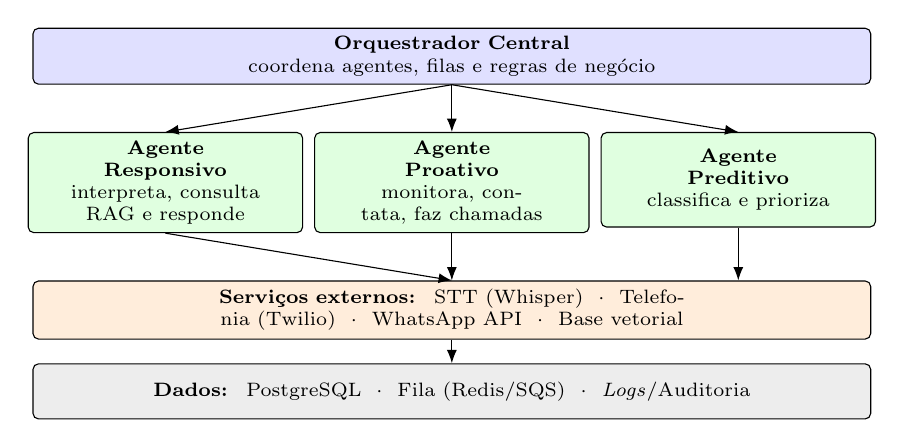
\begin{tikzpicture}[
  font=\scriptsize,
  box/.style={draw, rounded corners=2pt, align=center, minimum height=7mm, inner sep=3pt},
  orq/.style={box, fill=blue!12, text width=.86\linewidth},
  agent/.style={box, fill=green!12, text width=.27\linewidth, minimum height=12mm},
  serv/.style={box, fill=orange!14, text width=.86\linewidth},
  dados/.style={box, fill=gray!14, text width=.86\linewidth},
  >=Latex, node distance=3mm
]
\node[orq] (orq) {\textbf{Orquestrador Central}\\ \scriptsize coordena agentes, filas e regras de neg\'ocio};
\node[agent, below=6mm of orq.south, xshift=-.30\linewidth, anchor=north] (resp) {\textbf{Agente}\\\textbf{Responsivo}\\ \scriptsize interpreta, consulta RAG e responde};
\node[agent, below=6mm of orq.south, anchor=north] (proa) {\textbf{Agente}\\\textbf{Proativo}\\ \scriptsize monitora, contata, faz chamadas};
\node[agent, below=6mm of orq.south, xshift=.30\linewidth, anchor=north] (pred) {\textbf{Agente}\\\textbf{Preditivo}\\ \scriptsize classifica e prioriza};
\node[serv, below=6mm of proa] (serv) {\textbf{Servi\c{c}os externos:}~ STT (Whisper) ~$\cdot$~ Telefonia (Twilio) ~$\cdot$~ WhatsApp API ~$\cdot$~ Base vetorial};
\node[dados, below=3mm of serv] (dados) {\textbf{Dados:}~ PostgreSQL ~$\cdot$~ Fila (Redis/SQS) ~$\cdot$~ \textit{Logs}/Auditoria};
\draw[->] (orq.south) -- (resp.north);
\draw[->] (orq.south) -- (proa.north);
\draw[->] (orq.south) -- (pred.north);
\draw[->] (resp.south) -- (serv.north);
\draw[->] (proa.south) -- (serv.north);
\draw[->] (pred.south) -- ([xshift=.30\linewidth]serv.north);
\draw[->] (serv.south) -- (dados.north);
\end{tikzpicture}
\caption{Vis\~ao geral da arquitetura multiagente em quatro camadas.}
\label{fig:arquitetura}
\end{figure}

A coordena\c{c}\~ao entre os agentes ocorre por meio de uma fila de mensagens e eventos ass\'incronos, com regras de prioridade que privilegiam intera\c{c}\~oes responsivas (cliente aguardando) sobre as proativas, al\'em de pol\'iticas de escala\c{c}\~ao para atendimento humano. Todas as decis\~oes e intera\c{c}\~oes dos agentes s\~ao registradas em \textit{logs} de auditoria, atendendo a requisitos de rastreabilidade e de conformidade com a LGPD, incluindo a criptografia de dados pessoais em repouso.

A pilha tecnol\'ogica prevista \'e apresentada na Tabela~\ref{tab:stack}. O \textit{backend} adota Python com FastAPI em microsservi\c{c}os, separando a valida\c{c}\~ao de entrada da infer\^encia dos modelos. O m\'odulo preditivo emprega Random Forest e \textit{Gradient Boosting} (XGBoost) sobre \textit{scikit-learn}, servidos por uma API de infer\^encia dedicada. O RAG utiliza um banco vetorial (Qdrant ou \textit{pgvector}) e os agentes s\~ao orquestrados com LangGraph/LangChain. Os servi\c{c}os de voz combinam Whisper (transcri\c{c}\~ao) e ElevenLabs (s\'intese), integrados \`a telefonia program\'avel (Twilio/Vonage) e \`a WhatsApp Business API.

\begin{table}[t]
\centering
\small
\caption{Pilha tecnol\'ogica prevista.}
\label{tab:stack}
\begin{tblr}{
  width=\linewidth,
  colspec={Q[l]X[l]},
  row{1}={font=\bfseries},
  hline{1,2,Z}=0.6pt,
  rowsep=1.5pt,
}
Componente & Tecnologia \\
\textit{Backend}/API & Python + FastAPI (microsservi\c{c}os) \\
LLM & Claude / GPT-4 \\
\textit{Embeddings} & OpenAI / Sentence Transformers \\
Banco vetorial & Qdrant / \textit{pgvector} \\
ML & Random Forest / XGBoost (\textit{scikit-learn}) \\
Orquestra\c{c}\~ao de agentes & LangGraph / LangChain \\
Fila / Dados & Redis / AWS SQS $\cdot$ PostgreSQL \\
STT / TTS & Whisper $\cdot$ ElevenLabs \\
Telefonia & Twilio / Vonage \\
Mensageria & WhatsApp Business API \\
\end{tblr}
\end{table}

%% ============================================================
%%  4. RESULTADOS ESPERADOS
%% ============================================================
\section{Resultados Esperados}
\label{sec:resultados}

Esta se\c{c}\~ao descreve uma previs\~ao dos resultados, sujeita a ajustes at\'e o final do PAC 8. Para o m\'odulo preditivo, espera-se atingir, no conjunto de teste, F1-\textit{score} $\geq 0{,}75$, acur\'acia $\geq 0{,}80$ e AUC-ROC $\geq 0{,}80$ tanto na classifica\c{c}\~ao de propens\~ao ao pagamento quanto na previs\~ao de inadimpl\^encia futura, superando um \textit{baseline} de regress\~ao log\'istica simples. Para o m\'odulo responsivo, espera-se elevada fidelidade das respostas (ancoradas na base via RAG) e baixa taxa de alucina\c{c}\~ao, com tempo de resposta inferior a cinco segundos.

A qualidade do m\'odulo responsivo ser\'a medida em duas dimens\~oes: a do \textit{retrieval} (precis\~ao e revoca\c{c}\~ao em \textit{top-k}) e a das respostas geradas (relev\^ancia, fidelidade aos documentos, completude e taxa de alucina\c{c}\~ao), aferidas sobre um conjunto de perguntas de teste com respostas de refer\^encia.

No plano operacional, a hip\'otese ser\'a avaliada em um experimento controlado, comparando o sistema proposto a dois \textit{baselines} --- processo manual e processo semiautomatizado sem ML --- por um per\'iodo definido, com an\'alise estat\'istica dos indicadores quando o tamanho da amostra permitir. Esperam-se ganhos na \textbf{taxa de recupera\c{c}\~ao de cr\'edito} e redu\c{c}\~ao no \textbf{tempo m\'edio de resolu\c{c}\~ao} de pend\^encias, al\'em de maior \textbf{volume de atendimento simult\^aneo} (meta de pelo menos 100 intera\c{c}\~oes concorrentes) a um custo por contato inferior ao do atendimento humano. A prioriza\c{c}\~ao preditiva e a cobran\c{c}a preventiva devem antecipar a\c{c}\~oes e concentrar esfor\c{c}os nos contatos de maior retorno.

%% ============================================================
%%  5. DISCUSSÕES E CONCLUSÕES
%% ============================================================
\section{Discuss\~oes e Conclus\~oes}
\label{sec:discconclusao}

A proposta enfrenta desafios relevantes. No plano legal, a cobran\c{c}a automatizada deve observar o C\'odigo de Defesa do Consumidor \cite{cdc1990} e a Lei Geral de Prote\c{c}\~ao de Dados \cite{lgpd2018}, o que imp\~oe restri\c{c}\~oes de hor\'ario, frequ\^encia de contato, consentimento para grava\c{c}\~ao e prote\c{c}\~ao de dados pessoais. No plano t\'ecnico, destacam-se a lat\^encia em chamadas de voz com transcri\c{c}\~ao em tempo real, o risco de alucina\c{c}\~ao do LLM --- mitigado pelo RAG e por restri\c{c}\~oes de \textit{prompt} --- e o poss\'ivel desbalanceamento de classes nos dados de inadimpl\^encia, que demandar\'a t\'ecnicas como reamostragem ou pondera\c{c}\~ao de classes.

Um aspecto sens\'ivel \'e o equil\'ibrio entre automa\c{c}\~ao e empatia: a cobran\c{c}a lida com pessoas em situa\c{c}\~ao financeira delicada, de modo que o tom das mensagens, a transpar\^encia sobre a natureza automatizada do atendimento e o respeito imediato a pedidos de interrup\c{c}\~ao de contato s\~ao requisitos t\~ao importantes quanto o desempenho t\'ecnico. Decis\~oes preditivas tamb\'em exigem cuidado para n\~ao penalizar indevidamente determinados perfis de clientes, o que refor\c{c}a a import\^ancia da interpretabilidade dos modelos.

A proposta resolve a limita\c{c}\~ao de escala e de prioriza\c{c}\~ao do processo manual, unificando atendimento responsivo, abordagem proativa multicanal e intelig\^encia preditiva. N\~ao se prop\~oe, contudo, a substituir integralmente o operador humano: casos sens\'iveis e negocia\c{c}\~oes fora dos par\^ametros autom\'aticos permanecem sujeitos a escala\c{c}\~ao. S\~ao limita\c{c}\~oes previstas a depend\^encia de dados hist\'oricos de qualidade e os custos de APIs de LLM, voz e telefonia. Como trabalhos futuros, vislumbram-se a personaliza\c{c}\~ao de estrat\'egias por segmento de cliente, o uso de aprendizado por refor\c{c}o para otimizar pol\'iticas de contato e a expans\~ao a novos canais. Conclui-se que a integra\c{c}\~ao de LLMs com RAG, agentes aut\^onomos, modelos preditivos e servi\c{c}os de voz constitui um caminho promissor para automatizar e tornar mais eficiente o ciclo de recupera\c{c}\~ao de cr\'edito, hip\'otese a ser validada experimentalmente ao longo do PAC 8.

%% ============================================================
%%  6. APÊNDICE  (NÃO conta para o limite de páginas)
%% ============================================================
\section{Ap\^endice}
\label{sec:apendice}

Este ap\^endice re\'une a tabela comparativa de trabalhos relacionados (Tabela~\ref{tab:comparativa}) e o cronograma de desenvolvimento em semanas, da data atual at\'e o final do PAC 8 (Tabela~\ref{tab:cronograma}).

\begin{table*}[t]
\centering
\footnotesize
\caption{Tabela comparativa de trabalhos relacionados. Legenda: \atende{}~atende, \parcial{}~parcial, \naoatende{}~n\~ao atende; A1--A3 = artigos cient\'ificos, S1--S3 = solu\c{c}\~oes comerciais.}
\label{tab:comparativa}
\begin{tblr}{
  width=\textwidth,
  colspec={X[l]*{7}{Q[c,wd=1.05cm]}},
  row{1}={font=\bfseries,c},
  row{2}={font=\scriptsize\itshape,c},
  column{1}={l},
  rowsep=1.6pt,
  hline{1,3,Z}=0.6pt,
}
Crit\'erio & A1 & A2 & A3 & S1 & S2 & S3 & Prop. \\
 & Wang et al. (2024) & Mestiri (2024) & MASCA --- Jajoo et al. (2025) & HighRadius & Skit.ai & Tovie AI & Proposta do TCC \\
\SetCell[c=8]{l}\textit{Tecnologias de Intelig\^encia Artificial} & & & & & & & \\
P1 --- LLM (Modelo de Linguagem de Grande Escala) & \atende & \naoatende & \atende & \parcial & \atende & \atende & \atende \\
P2 --- RAG (\textit{Retrieval-Augmented Generation}) & \naoatende & \naoatende & \parcial & \naoatende & \naoatende & \naoatende & \atende \\
P3 --- Modelos preditivos de \textit{Machine Learning} & \naoatende & \atende & \parcial & \atende & \parcial & \parcial & \atende \\
P4 --- Arquitetura multiagente & \atende & \naoatende & \atende & \naoatende & \naoatende & \naoatende & \atende \\
\SetCell[c=8]{l}\textit{Canais de Comunica\c{c}\~ao} & & & & & & & \\
P5 --- Opera\c{c}\~ao multicanal (texto + voz) & \naoatende & \naoatende & \naoatende & \atende & \atende & \atende & \atende \\
P6 --- Integra\c{c}\~ao com telefonia program\'avel & \naoatende & \naoatende & \naoatende & \naoatende & \atende & \atende & \atende \\
P7 --- Transcri\c{c}\~ao autom\'atica de fala (STT) & \naoatende & \naoatende & \naoatende & \naoatende & \atende & \atende & \atende \\
\SetCell[c=8]{l}\textit{Estrat\'egia de Cobran\c{c}a} & & & & & & & \\
P8 --- Abordagem proativa aut\^onoma & \parcial & \naoatende & \naoatende & \atende & \atende & \atende & \atende \\
P9 --- Atendimento responsivo ao cliente & \parcial & \naoatende & \naoatende & \parcial & \atende & \atende & \atende \\
P10 --- Prioriza\c{c}\~ao inteligente de inadimplentes & \naoatende & \parcial & \atende & \atende & \parcial & \parcial & \atende \\
P11 --- Cobran\c{c}a preventiva (inadimpl\^encia futura) & \naoatende & \naoatende & \naoatende & \parcial & \naoatende & \naoatende & \atende \\
\SetCell[c=8]{l}\textit{Dom\'inio de Aplica\c{c}\~ao} & & & & & & & \\
P12 --- Foco espec\'ifico em cobran\c{c}a e recupera\c{c}\~ao de cr\'edito & \naoatende & \parcial & \atende & \atende & \atende & \atende & \atende \\
\textbf{Pontua\c{c}\~ao total (m\'ax. 12,0)} & 3,0 & 2,0 & 5,0 & 6,5 & 8,0 & 8,0 & \textbf{12,0} \\
\textbf{Cobertura dos requisitos (\%)} & 25\% & 17\% & 42\% & 54\% & 67\% & 67\% & \textbf{100\%} \\
\end{tblr}
\end{table*}

\begin{table}[t]
\centering
\small
\caption{Cronograma de desenvolvimento em semanas (jun.\ a dez.\ de 2026).}
\label{tab:cronograma}
\begin{tblr}{
  width=\linewidth,
  colspec={Q[l,wd=1.4cm]X[l]},
  row{1}={font=\bfseries},
  hline{1,2,Z}=0.6pt,
  rowsep=1.5pt,
}
Semanas & Etapa \\
1--2 & Requisitos e an\'alise do dom\'inio (LGPD/CDC) \\
3--5 & Coleta e prepara\c{c}\~ao de dados (EDA, \textit{feature engineering}) \\
6--9 & M\'odulo preditivo de ML (treino, avalia\c{c}\~ao, API) \\
8--11 & Arquitetura multiagente e orquestrador \\
10--14 & M\'odulo responsivo (RAG + LLM) \\
13--17 & M\'odulo ativo/proativo (agentes, WhatsApp, regras) \\
16--19 & Integra\c{c}\~ao de voz (STT/TTS, telefonia) \\
19--22 & Testes, experimentos e avalia\c{c}\~ao \\
22--24 & Reda\c{c}\~ao final e prepara\c{c}\~ao da defesa \\
\end{tblr}
\end{table}

%% Garante que as tabelas flutuantes do Ap\^endice sejam totalmente posicionadas
%% ANTES das Refer\^encias, evitando que a bibliografia seja intercalada com as tabelas.
\clearpage

\bibliographystyle{apalike-sol}
\bibliography{refs}

\end{document}
